\section{Durchführung}
\label{sec:Durchführung}
\subsection{Aufbau}
Der Aufbau ist in Abbildung \ref{fig:Aufbau} zu sehen, im gegebenen Versuch wurde kein Plastikzylinder verwendet.
Der Aufbau besteht aus einem Messingzylinder in einem Helmholtzspulenpaar mit Windungszahl $N = 195$ Abstand $d = 0.138$m Radius $R = 0.109$m. Auf dem messingzylinder befindet sich eine Billardkugel mit Masse $m = 150g$ und Rasius $R = 0.028$m mit einem Magenten in ihrem inneren, und einem Stiel in Richtung des magnetischen Momentes.
Für die ersten beiden messreihen steckt in dem Stiel ein Aluminiumstab an dem im Abstand $r$ ein Gewicht der Masse $m = 1.4$g. Über dem Zylinder ist ein Stroboskop angebracht. Der Aufbau verfügt des weiteren über ein Steuergerät mit dem das Magentfeld der Helmholtzspulen, 
das Stroboskop und ein Luftkissen im Messingzylinder bedient werden können.
\subsection{Messung zur Bestimmung des magnetischen Momentes durch Gravitation}
Die Masse am Aluminiumstab wird um eine bestimmte Länge $r$ am Aluminiumstab von der Kugel entfernt. Das Luftkissen wird eingeschaltet, und das Magnetfeld der Helmholtzspulen wird durch die Stromstärke $I$ so reguliert,
dass sich das gewicht im Gleichgewicht befindet, Es werden 10 Messwerte Paare $r,I$ aufgenommen.
\subsection{Messung zur Bestimmung des magnetsichen Momenetes durch Oszillation}
Das gewicht am Aluminiumstab wird nun entfernt, die kugel wird in Ruheposition verstzt, und dann anschliessen um einen kleinen Winkel ausgelenkt. An der Steuereinrichtung wird ein bestimmtes $I$ eingestellt. Das Luftkissen wird angeschaltet, und es werden 10 Schwingungsperioden $T$ der Kugel mithilfe einer Stoppuhr gemessen, es werden 10 verschiedene Messwerte Paare $I,10T$
mit unterschiedlichen Stromstärken aufgenommen.
\subsection{Messung zur Bestimmung des magnetischen Momentes über Präzession eines Magneten}
Nun wird auch der Aluminiumstab entfernt, das Stroboskop wird mit gleich bleibender Frequenz $F = 4.2$Hz betrieben. Bei eingeschaltetem Luftkissen wird die Kugel
 von Hand in Drehung versetzt. Sobald der weiße Punkt auf dem Stiel beim Lichtblitz immer am selben ort erscheint, wird die Drehfrequenz als gleich der Stroboskopfrequenz angenommen, und die Stromstärke $I$ wird eingeschaltet, es wird eine Periode der nun auftretenden Präzession mithilfe der Stoppuhr gemessen. 
 Dies wird für jede Stromstärke drei mal durchgeführt, insgesamt wird für 5 verschiedene Stromstärken gemessen.

\begin{figure}
    \centering
    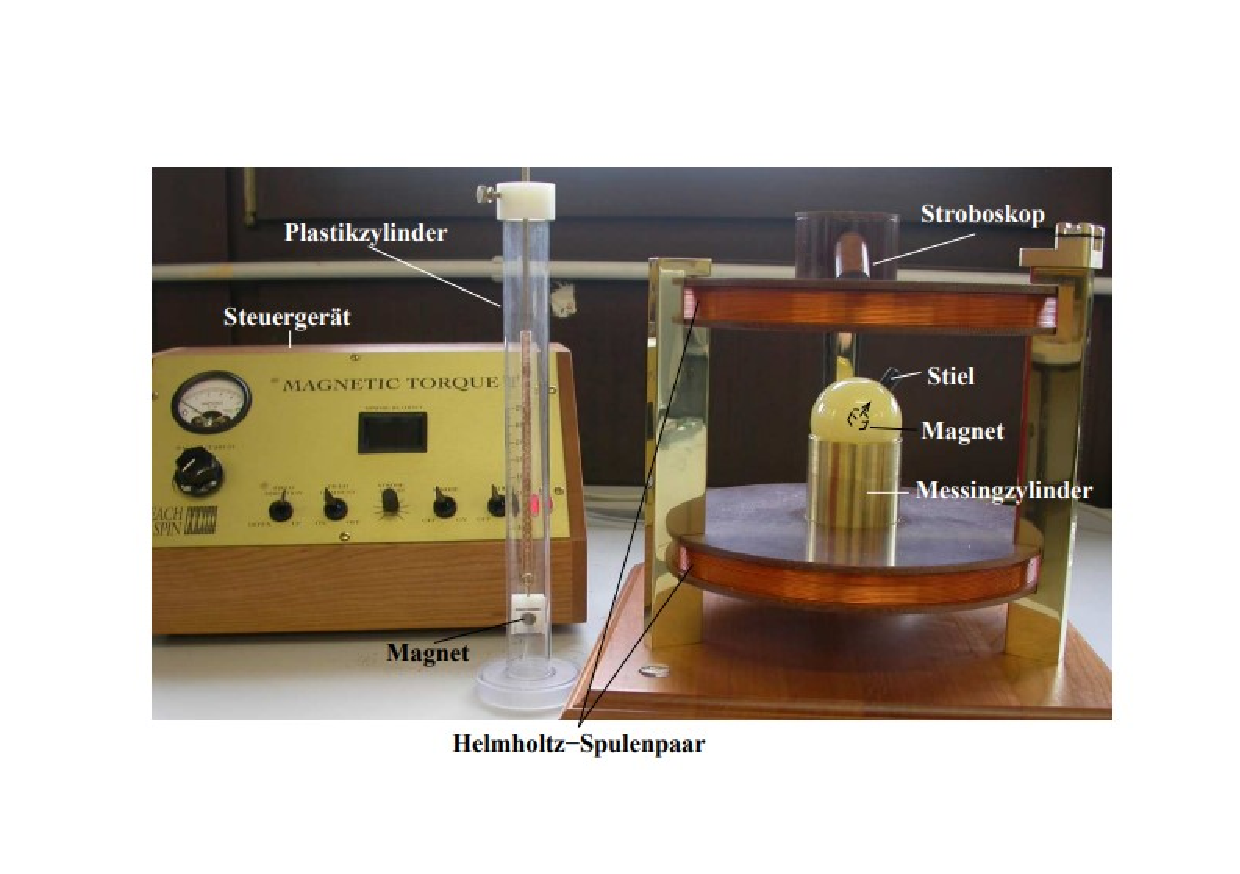
\includegraphics[width = 15cm]{V105Aufbau.pdf}
    \caption{Versuchsaufbau \cite{V105}}
    \label{fig:Aufbau}
\end{figure}